\chapter{Introduction}
     
The invention of the integrated circuit in the late 1950’s can be considered a milestone in modern technology and a start of a new period in modern society: The age of silicon. With the ever-increasing demand for fast, compact, and more efficient electronic devices, there seems to be no slowing down for the development of novel materials such that scaling (reduction of transistor feature size) can continue to support Moore’s Law. Loosely speaking, Moore’s Law (or observation) states that the number of transistors on an integrated circuit doubles approximately every two years (Moore’s original paper actually described the economics of scaling and the minimum cost per component \cite{moore1998}). Moore's law scaling is typically reserved to describe scaling of computational elements such as metal-organic-semiconductor field-effect transistors (MOSFETs), but memory elements such as dynamic random access memory (DRAM) capacitors experience rapid scaling as well \cite{Kim2008}.

The perpetuation of Moore's law has largely been possible due to continued materials research and development. These developments include the ability to grow pristine single crystalline semiconductors, control the chemistry of the semiconductors through doping, and grow high quality oxides on the semiconductors. The ability to grow high quality amorphous gate oxides with low defect densities (on the order of 10$^{10}$/cm$^{2}$ \cite{Wilk2001}) is especially important and arguably the major reason silicon has reigned supreme in the semiconductor industry. However, persistent scaling of transistor size introduced a series of problems. One of the ``grand challenges" at the turn of the century for the semiconductor industry was finding a suitable replacement for SiO$_{2}$ \cite{roadmap1997}.

The critical issue with SiO$_{2}$ transistor scaling is the tunneling of electrons through the gate oxide, which is akin to the tunneling of a particle wavefunction through a finite potential barrier. As we know from quantum mechanics, the probability of the particle wavefunction seeping or ``tunneling" through the finite barrier scales exponentially with barrier thickness; a thinner barrier will result in a higher tunneling probability. 

The theories that model electron conduction through an oxide have been around for quite a while. For example, calculations performed by Snow and Lenzlinger in the late 60s show that electrons tunneling through a triangular potential barrier follow Fowler-Nordheim tunneling \cite{Lenzlinger1969}. The problem with this model is that oxides back then were generally much thicker ($\sim$1000 \AA), in comparison to gate oxides today (sub-100 \AA) and at these length scales a full quantum mechanical treatment is necessary. More recently, quantum mechanical modeling of electron conduction through SiO$_{2}$ was carried out by Lo et al., and they showed that the gate oxide could scale to 20 \AA\;before tunneling currents became a problem \cite{Lo1997}. The ultimate limit to the scaling of SiO$_2$ before it becomes an incontrovertible problem is still under debate. However, recently Muller et al. showed using electron energy loss spectroscopy (EELS) that a significant fraction of the gate oxide consists of interfacial sub-oxide having properties that are different from the bulk, reducing the limit to about 1.2 nm for silicon oxide \cite{Muller1999}.

Finding a replacement for SiO$_{2}$ involved balancing several stringent material requirements \cite{Wilk2001,Robertson2006}, the most critical being the reduction of tunneling currents. Since the tunneling current depends on barrier thickness, an obvious solution is to introduce a thicker gate oxide. We can model the gate oxide as a parallel plate capacitor with gate capacitance, $C_{gate}$:
\begin{equation}\label{eq:gateC}
C_{gate} = \frac{\varepsilon_{0}\varepsilon_{r}A}{t}
\end{equation}
where $\varepsilon_{0}$ is the permittivity of free space, $\varepsilon_{r}$ the relative permittivity (also known as k or $\kappa$, hereupon used interchangeably), $A$ is the area, and $t$ is the thickness of the oxide. Increasing the thickness $t$ requires that one either increase $A$ or $\varepsilon_{r}$ in order to keep the capacitance constant. Increasing $A$ would defeat the point of transistor scaling, hence increasing $\varepsilon_{r}$ is the obvious choice. Materials with $\varepsilon_{r}$ that are higher than SiO$_{2}$ have become known colloquially as ``high-k" dielectrics. 

It is convenient to define an equivalent oxide thickness $t_{eq}$ (EOT):
\begin{equation}\label{eq:teq}
t_{eq} = \left(\frac{3.9}{k}\right) t_{high-\kappa}
\end{equation} 
to facilitate the comparison of oxides of different compositions. Using this parameter one can calculate the thickness of SiO$_{2}$ that would achieve an equivalent areal capacitance in comparison to a material with a higher dielectric constant. For instance, if we had a material with a dielectric constant of 39 and $t_{high-\kappa}$ of 40 \AA, one could in theory achieve areal capacitances that would be equivalent to using SiO$_{2}$ that is 4 \AA\,thick. In reality the dielectric does not scale linearly and one has to consider depletion and quantum mechanical effects that can change the effective oxide thickness. 

It turns out that it is insufficient to simply increase the dielectric constant of the oxide to reduce tunneling currents. In addition to the dielectric constant, one must also consider the band offsets between the semiconductor and the oxide to prevent Schottky emission of electrons and holes into the oxide bands \cite{Robertson2000}. This is illustrated in the following relation for the tunneling current expressed in the direct tunneling regime \cite{Yeo2000}. In simplified form \cite{Yeo2002a} the tunneling current is,
\begin{equation}\label{eq:JT}
J \sim \text{exp}\left(-\frac{8\pi\sqrt{2q}}{3h} (m_{\text{eff}}\,\phi_{b})^{0.5} \kappa\;t_{eq}\right)
\end{equation}
where $q$ is the charge, $h$ is Planck's constant, $m_{\text{eff}}$ is the effective mass, $\phi_{b}$ is the barrier height, $\kappa$ is the dielectric constant, and $t_{eq}$ is the equivalent thickness. The tunneling current $J$ is a function of  $\phi_{b}$ and $\kappa$ so the appropriate figure of merit for the tunneling current is the product $\phi_{b}^{0.5}\kappa$. 

\begin{figure}[ht]
\centering
\noindent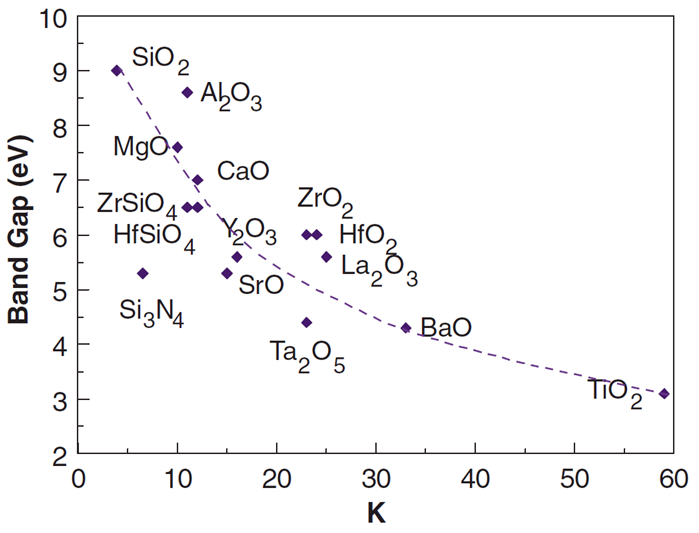
\includegraphics[width=0.7\textwidth]{chapter_1/bandgapvsk}
\caption{Band gap versus dielectric constant for potential high-k gate dielectrics.}
\label{fg:bandgapvsk}
\end{figure}

To demonstrate this point, it is useful to plot the dielectric constant versus band gap (Figure \ref{fg:bandgapvsk}) \cite{Robertson2008}. Figure \ref{fg:bandgapvsk} reveals a roughly inverse dependence on $\varepsilon_{r}$. Assuming that the band gaps align symmetrically with respect to silicon, this means that oxides with larger dielectric constants will likely have a smaller barrier height and are susceptible to leakage currents by Schottky emission. This suggests that dielectrics such as TiO$_{2}$ \cite{Kim2004}, BaTiO$_{3}$ \cite{Arlt1985}, and BaSrTiO3 \cite{Horikawa1993, Hilton1996} may not be suitable alternatives, even though they exhibit very high dielectric constants. In general the conduction band offset is much smaller than the valence band offset, so it is more instructive to plot the dielectric constant as a function of conduction and valence band offsets (Figure \ref{bandoffsetvsk}) \cite{Robertson2008}. Ideally, a band offset of at least 1 eV is desirable. In Figure \ref{bandoffsetvsk} we see that La based group III oxides exhibit a good balance of both high dielectric constant and band offset. Indeed, materials such as LaAlO$_{3}$ \cite{Edge2006} and LaLuO$_{3}$ \cite{Liu2011} show promise as potential high-k gate dielectrics. 

\begin{figure}
\centering
\noindent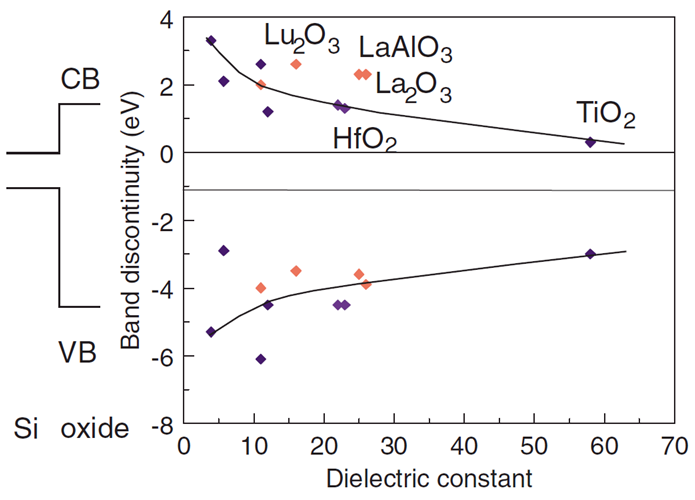
\includegraphics[width=0.7\textwidth]{chapter_1/bandoffsetvsk}
\caption{Measured band offsets of oxides on Si against dielectric constant for candidate gate oxides. Group III oxides are shown in red, HfO$_{2}$ and ZrO$_{2}$ in blue. From Reference \cite{Robertson2008}.}
\label{bandoffsetvsk}
\end{figure}

Other critical factors include interface quality and the thermodynamic and kinetic stability of the oxide in contact with the channel material and the gate electrode. Many potential candidates for gate oxides such as Ta$_{2}$O$_{5}$ and TiO$_{2}$ were initially adopted from DRAM technology \cite{Chaneliere1998,Kingon2000}; however, many turned out to be incompatible as gate oxides due to thermodynamic incompatibility with Si \cite{Hubbard1996a, Schlom2002}. Achieving a good interface and minimizing the defect densities at the oxide-semiconductor interface is also of paramount concern to abate deleterious effects such as charge trapping, which can decrease the carrier mobility in the channel and also cause Fermi level pinning.

\section{Amorphous transition metal-oxide dielectrics}

In the search for a suitable replacement to SiO$_{2}$, one consideration is whether to use an amorphous or crystalline material for the gate oxide. The advantage of amorphous materials is the lack of grain boundaries found in polycrystalline materials, which can act as sites for leakage currents to flow. In addition, the applied field will be uniform across the gate because the dielectric constant does not change with crystal orientation of the dielectric. Note, epitaxial growth of single crystalline oxides can also circumvent the problem of grain boundaries and is currently an area of active research \cite{dai2003}.

The challenge with amorphous materials is that many of the potential high-k gate oxides, such as HfO$_{2}$ and ZrO$_{2}$, crystallize at temperatures required to activate implanted dopants in the channel ($\sim$1000 \textdegree C). Crystallization of the oxide can be suppressed by doping silicates, but this comes at the cost of a lowered dielectric constant \cite{VanDover2003}. A surprising result showing an enhanced dielectric constant for zirconium and hafnium silicates at low SiO$_{2}$ concentrations \cite{Wilk2000, Wilk2000a}, demonstrated the possibility of evading the low-k problem. The result also initiated a slew of experimental and computational attempts to explain the anomalous effect, as it is a peculiar result in amorphous systems. Ultimately, the enhanced dielectric constants were not consistently reproducible \cite{Rignanese2002, Pignedoli2007}, nonetheless it remains to be an interesting theoretical and computational problem. In the following section we provide efforts to understand this anomalous dielectric phenomena in amorphous Hf-Si-O and Zr-Si-O.

\subsection{Dielectric anomalies in amorphous Hf-Si-O and Zr-Si-O dielectrics}

In 2007, Intel announced the introduction of their new transistor incorporating a HfO$_{2}$ $\emph{based}$ gate oxide and a metal gate electrode \cite{Mistry2007}. Work leading up to this involved countless attempts to screen various oxides. From the start a prime candidate was transition metal silicates. The rationale behind the silicates was to compromise a ``high" dielectric constant oxide ($\varepsilon_{r} \sim 22$ for HfO$_{2}$) in exchange for interface quality by doping SiO$_{2}$. Initial results for Hf-Si-O and Zr-Si-O were very promising; the oxides did not react in direct contact with Si up to at least 1050 \textdegree C, leakage currents were less than $\sim$10$^{-6}$ A/cm$^{-2}$ with high breakdown fields on the order of 10 MV/cm \cite{Wilk2000a}. There was evidence that silicates with higher concentrations of transition metal oxide were susceptible to crystallization at lower temperatures  ($<$1000 \textdegree C) \cite{Neumayer2001}, but the addition of nitrogen in the metal silicate was shown to improve thermal stability of the material \cite{Visokay2002}.

The surprising feature is arguably the unexpected enhancement in the dielectric constant. Referring to the original work by Wilk \cite{Wilk2000a}, a simple calculation reveals that the expected value for $\varepsilon_{r}$ with x $\sim$ 17 at.\% Hf in Hf$_{x}$Si$_{1-x}$O$_{2}$ (again, assuming $\varepsilon_{r} \sim 22$ for HfO$_{2}$ and $\varepsilon_{r} \sim 3.9 $ for SiO$_{2}$) is $\sim7$. The authors however report a value of $\varepsilon_{r}$ $\sim$ 11, which is about a 60\% increase from the expected value based on a weighted mean of the metal oxide concentrations. A similar effect is observed for zirconium silicates, denoting their chemical similarities.  

Dielectric enhancement is not unheard of, especially in crystalline form. For example, work by Cava showed that substitution of \ce{TiO2} in \ce{Ta2O5} stabilizes the H' monoclinic phase resulting in a near four-fold increase in the dielectric constant \cite{Cava1995}. A similar approach can be taken for Hf and Zr based oxides, where a high temperature phase (tetragonal or cubic) can be stabilized at room temperature to increase the dielectric constant \cite{Chalker2008a, Fischer2008b, Park2006}. A perfect demonstration of this is the stabilization of tetragonal \ce{HfO2} by substitution of 5 atomic percent \ce{SiO2} followed by a high temperature anneal. Here, the authors report a maximum $\kappa$ value of 27, versus an amorphous value of $\kappa \sim 20 $ \cite{Tomida2006}.

The relationship between the dielectric constant and structure is more tenuous. This of course is not to say that it is impossible to form a relationship between the two, and several experimental and theoretical developments are available on this front for hafnium and zirconium silicates. Initial studies utilizing Fourier Transform Infrared Spectroscopy (FTIR) suggested that the enhancement was due to four-fold coordinated Zr-O bonds \cite{Lucovsky2000}. In contrast, cluster simulations performed by Kurtz and Devine revealed the energetic stability of six-coordinated Zr over four \cite{Kurtz2001}. A six-coordinated Zr cluster would infer a higher local network density, a smaller molar volume, and thus a higher dielectric constant according to the Clausius-Mossotti relation \cite{Kurtz2001}. Calculations by Rigananese et al. related the dielectric constant of Zr-Si-O to local structural units \cite{Rignanese2002}. A modest enhancement of $\epsilon_{r}$ was attributed to ZrO$_{6}$ octahedra, but was not sufficient to account for the large reported enhancement in $\varepsilon_{r}$. Recent large-scale \textit{ab initio} simulations suggest that the inconsistent data for $\varepsilon_{r} (x)$ in amorphous $\textnormal{Zr}_{x}\textnormal{Si}_{1-x}\textnormal{O}_{2}$ and $\textnormal{Hf}_{x}\textnormal{Si}_{1-x}\textnormal{O}_{2}$ is due to variability in local structure associated with the variety of coordination numbers accommodated by the transition metal \cite{Pignedoli2007}.  In that work it was also found that a correlation between $\varepsilon_{r}$ and density could not be established, refuting earlier models for dielectric enhancement based solely on changes in density \cite{Kurtz2001,Devine2001}.

The nontrivial dependence of the dielectric constant of Hf(Zr)-Si-O on local structure clearly indicates a wealth of scientific knowledge that can be gained from studying complex amorphous materials. Next, we present a more recent discovery of a tantalum based amorphous oxide exhibiting anomalous dielectric properties similar to those observed in the Hf(Zr)-Si-O system. These results lead us to believe that this type of behavior is not entirely unique and that there are other amorphous systems which can exhibit unusual properties.

\subsection{Tantalum based amorphous materials and anomalous behavior in Ta-Ge-O}

Tantalum pentoxide is a dielectric material that is used in a variety of technological applications including DRAM memory, antireflective coatings, and the more nascent non-volatile memories \cite{Chaneliere1998, Banno2010}. Structurally, the material is quite complex, with the existence of many polymorphic structures. This is partly due to \ce{Ta}'s large coordination number which can range from six to as large as eight oxygen atoms \cite{Fukumoto1997, Liu2007b}.  Because of this complex structural morphology, it is of great computational and experimental interest \cite{Kimura1995a,Andreoni2010, Bassiri2011, Lee2013}.
\begin{figure}[ht]
\centering
\noindent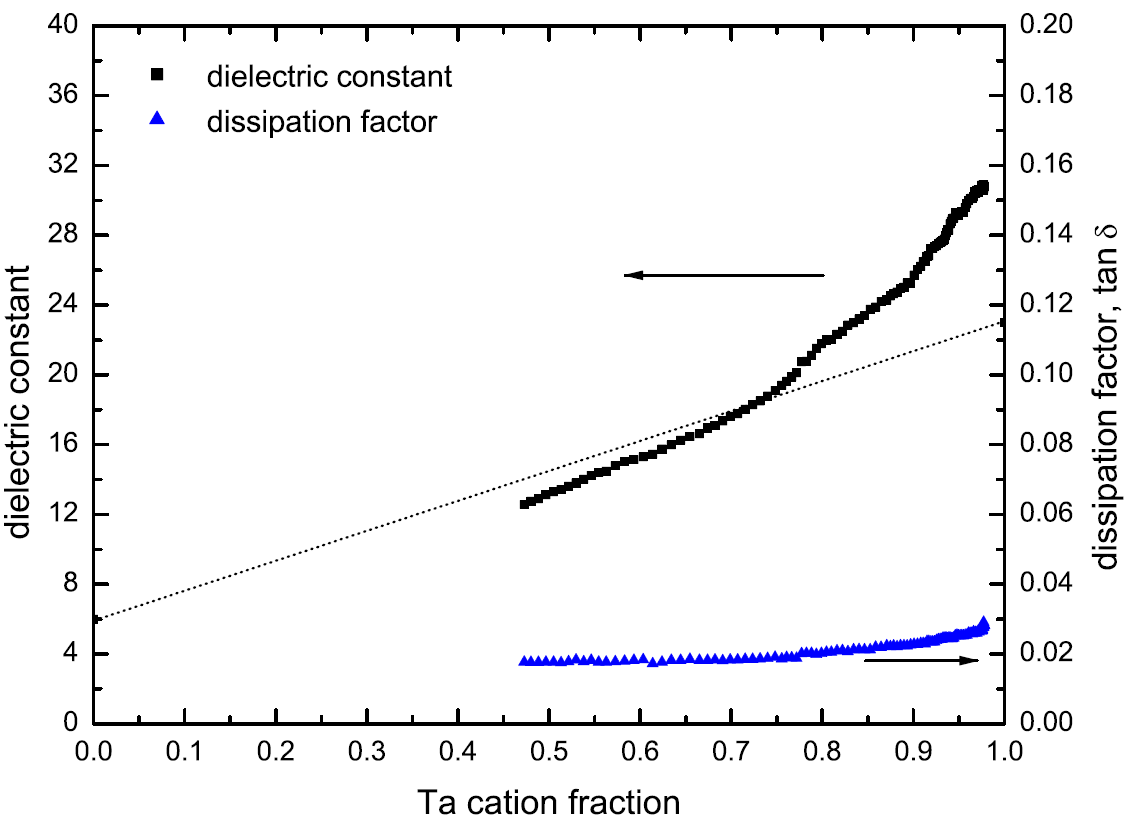
\includegraphics[width=0.7\textwidth]{chapter_1/tageox}
\caption{The variation in dielectric constant (black squares) and dissipation factor (tan d, blue triangles) of Ta$_{x}$Ge$_{1-x}$O$_{y}$ as a function of Ta cation fraction measured at 10 kHz. The dotted line represents the linear interpolation between endmember values. The uncertainty in $\varepsilon_{r}$ is estimated to be $\pm$ 5$\%$, dominated by uncertainty in the ellipsometrically determined thickness. From Reference \cite{Naoi2012}.}
\label{tageox}
\end{figure}

It was recently reported that mixed amorphous tantalum germanium oxide exhibits a dielectric constant, $\varepsilon_{r}$ as much as 40\% higher than that of pure tantalum oxide (Figure \ref{tageox}) \cite{Naoi2012}. Moreover, the dielectric constant exceeds the value of both pure \ce{Ta2O5} and \ce{GeO2}. This was not the case for the Hf(Zr) silicates, in which the dielectric constant only exceeded the value of the lower endmember \ce{SiO2}. Currently there is no coherent rationale which explains this behavior. Through this dissertation we wish to study this material system further in order to understand the underlying mechanisms which give rise to this phenomenon.

\section{Alternative computing and memory architectures: Motivation to study thin film complex amorphous oxides}

It is clear that sooner or later Moore's law scaling will come to an end or need to be completely redefined due to physical limitations or simply becoming too impractical to pursue. In anticipation of this impending limitation, different avenues are already being explored. These include, but are not limited to, advancement in 3D transistors \cite{Hisamoto2000}, quantum computing \cite{Devoret2013}, and neuromorphic computing \cite{Pershin2012}. Similar trends are being pursued in memory storage architectures, which emphasize non-volatile forms of memory \cite{Meijer2008}.

Memory devices expectedly stress different requirements in comparison to logic devices. These are things such as read/write (R/W) times, retention time, number of cycles the memory can endure, energy required to flip the bit, and the maximum achievable memory density. Current R/W times for Hard disk drives (HDDs) are on the order of several milliseconds (Table \ref{table:memory}). Solid state drives based on Flash(NAND) memory improve R/W times by an order of magnitude or two, but still suffer from low endurance (10$^{4}$ cycles). On the other hand, the switching speeds of DRAM capacitors are extremely fast---on the scale of tens of nanoseconds---in addition to exhibiting cycle endurances greater than 10$^{16}$. The clear drawback however, is the ephemeral nature of the memory (retention time $<<$ seconds), since DRAM is not designed for long term memory storage. Comparisons of HDD/Flash memory versus DRAM illustrate the historical trend for memory devices to either sacrifice R/W speeds for retention time or retention time for R/W speeds. Emerging memory technologies such as phase change memory (PCM) and spin torque transfer random access memory (STTRAM) attempt to eliminate the need for this trade-off.

\begin{table}
\centering
\scriptsize
\begin{tabular}{llllllll}
\toprule
& \textbf{Memristor} & \textbf{PCM} & \textbf{STTRAM} & \textbf{SRAM} & \textbf{DRAM} & \textbf{Flash(NAND)} & \textbf{HDD}\\
\midrule
&&\multicolumn{2}{c}{\textbf{Prototype}}& \multicolumn{4}{c}{\textbf{Commercialized technologies}} \\
\cmidrule(lr){3-4} \cmidrule(lr){5-8} 
Reciprocal density (F$^{2}$)  & $<$ 4 & 4-16 & 20-60 & 140 & 6-12 & 1-4 & 2/3 \\
Energy per bit (pJ) & 0.1-3 & 2-25 & 0.1-2.5 & 0.0005 & 0.005 & 0.00002 & 1-10$\times$10$^{9}$  \\
Read time (ns) &  $<$10 & 10-50 & 10-35 & 0.1-0.3 & 10 & 100,000 & 5-8$\times$10$^{6}$\\
Write time (ns) & $\sim$10 & 50-500 & 10-90 & 0.1-0.3 & 10 & 100,000 & 5-8$\times$10$^{6}$ \\
Retention time & years & years & years & As long as & $<<$ second & years & years \\
&&&&voltage &&&\\
&&&&applied&&&\\
Endurance (cycles) &10$^{12}$&10$^{9}$&10$^{15}$&$>$10$^{16}$&$>$10$^{16}$&10$^{4}$&10$^{4}$\\
\bottomrule
\end{tabular}
\caption{Comparison of current memory storage technologies. PCM, phase change memory; STTRAM, spin torque transfer random access memory; SRAM, static RAM, DRAM, dynamic RAM; HDD, hard disk drive. Taken from Reference \cite{Yang2013}.}
\label{table:memory}
\end{table}

On this front, electrical switches that utilize resistance change to store and perform logic operations (e.g. memristors) are most promising \cite{Yang2013}. The concept of switching and memory phenomena involving the differential change in materials resistance has been known for some time \cite{Dearnaley1970}. But recent improvements in the ability to probe materials at the nanoscale have facilitated the observation of microscopic changes in the material with switching. One can also draw from the vast knowledge of device processing accumulated over the years to scale devices down to improve memory density. The challenge now, is to gain a deeper understanding of the switching phenomena and relate the structural changes that occur with the electrical properties of the material in order to design suitable materials. 

Many resistive materials which display switching behavior start amorphous (mixed amorphous/polycrystalline in the work by Kwon et al.) \cite{Yao2010a, Kwon2010a, Lee2011a}, which is equivalent to a ``0".  The material is switched to the ``on" state, equivalent to a ``1," when a conductive crystalline pathway forms between the electrodes. The exact mechanism for the switching behavior is still under debate \cite{Yang2013}, but an understanding of the amorphous structure of amorphous oxides can provide insight into the behavior of such devices. Furthermore, current resistive materials often utilize binary oxides, and thus the resistive behavior of more complex compositions is not very well understood. To characterize the resistive behavior of complex amorphous oxides, multi-component sputtering may prove to be useful. 

\section{Deposition technique: off-axis sputtering for multi-composition research}

The majority of thin film samples in this work were deposited using RF magnetron sputtering. When considering thin film deposition techniques for creating complex amorphous oxides, sputtering provides several advantages over other deposition techniques which are more commonly found in large scale industrial fabs, namely chemical vapor deposition (CVD) and its close cousin, atomic layer deposition (ALD). CVD methods depend on the thermodynamic reactions between volatile precursors. Therefore, film stoichiometry is strongly predicated on the capacity to control the reaction between precursors using various annealing and gas transport processes. This makes CVD type methods suitable for tightly controlling the stoichiometry of uniform films, but unfit for combinatorial depositions that require depositing many compositions in one run. 

Sputtering, in contrast, involves the volatilization of pure metal or ceramic compounds using a plasma, allowing for the deposition of high purity films. When metal targets are used, high purity oxygen is introduced into the chamber to oxidize the volatilized metals. Film stoichiometry can be readily varied across a film in a single run by depositing composition spreads \cite{VanDover2004a}. This is achieved in our lab by orienting the sputtering guns in an oblique configuration, as shown in Figure \ref{fenris}.

\begin{figure}
\centering
\noindent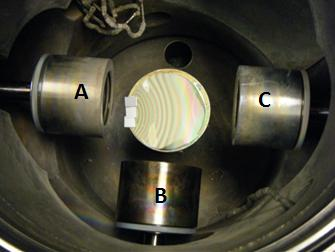
\includegraphics[width=0.7\textwidth]{chapter_1/fenris}
\caption{Top down view inside the sputtering chamber that is used in this work. Three magnetron sputtering guns are in the 90 degree off-axis configuration with respect to the substrate. Sputtering in this configuration results in a natural thickness gradient across the substrate. Guns A, B, and C can be energized simultaneously to create a composition spread.}
\label{fenris}
\end{figure}

When the targets are sputtered in this configuration a natural thickness gradient is obtained across the substrate. Due to the formation of a natural thickness gradient, sputtering from two or more targets simultaneously will also result in a natural composition gradient. The added bonus here is that the sputtered constituents are intimately intermixed, i.e. the atoms form a true atomic scale amorphous mixture. To achieve a similar effect using ALD would be cumbersome since it is a technique that involves layer by layer growth. Also in comparison to discrete combinatorial methods \cite{Xiang1995} the composition resolution of continuous composition methods is much finer, on the order of $\sim$ 0.1 mol\% \cite{VanDover2004a}.

The disadvantage of sputtering is that the sputtering can introduce defects and inclusions in the thin film. Not surprisingly the most common inclusion is Ar for sputtering \cite{Cuomo1977}. There is also the effect of introducing substantial film stress in the film if the substrates are biased during the deposition \cite{Kim1998}. Nonetheless, applying a substrate bias is a necessary process during off-axis deposition to preclude the formation of columnar voids \cite{Barron2009}. Finally, because sputtering is a line of sight deposition technique, it is not suitable for depositions that require high conformity to the surface topology of the device. Ultimately, the utility of the materials discovered and evaluated using the composition spread methods needs to be compatible with deposition techniques used in industry. 
